\documentclass[a4paper,11pt,titlepage]{article}

\usepackage{listings}
\usepackage{amsmath}
\usepackage{amssymb}
\usepackage{amsthm}
\usepackage{graphicx}
\usepackage{hyperref}
\usepackage{parskip}

\setlength{\parindent}{15pt}
\setlength{\emergencystretch}{3em}

\begin{document}

\title{Multi-pose people detection in 3D point clouds}
\author{Stefano Zanella - 621796}
\date{Feb 2017}

\maketitle

\section{Abstract}
This paper describes a people detection algorithm for three-dimensional point
clouds based on the well-known Viola-Jones face recognition algorithm (Viola and
Jones, 2003). The key contribution of the project is an implementation of
mentioned algorithm, adapted for work with 3D point clouds. The implementation
consists in a cascaded classifier and its training algorithm. This detector
serves as a cornerstone for the overall people detection algorithm, which
features a variant of the region-growing segmentation algorithm found in the PCL
library. Analysis of the algorithm's performance are provided based on a
given set of 40 images.

\newpage

\section{Introduction}
This paper attempts at extending the current research in the field of
recognition of human beings in three-dimensional point clouds. The key intuition
behind the proposed approach is that human presence in a scene might be
connected to the presence of any part of a human body.

Building a detector flexible enough to recognize any body part (e.g. a face or a
hand), or any sensible combination of them (e.g. a leg and a foot), is a task
that has low chances to lead to good performances. Indeed, also designing a
detector that recognizes bodies in multiple poses is not a simple task, as the
flexibility of human body makes the number of possible poses very high. \\
Moreover, such a detector might not perform well in case of obstructed bodies or
bodies only partially framed into the scene.

Therefore, the proposed approach starts from the most distinguishing part of
a human body: its head. A human head, put in the context of a larger scene,
provides some desirable features:

\begin{itemize}
  \item it's relatively rigid, meaning that it acts approximately as any other rigid
  body that can only be subject to rotation. This is important as it allows to
  be detected by using standard object recognition techniques
  \item it's small compared to the rest of the body, opening the door to algorithms
  that achieve higher performances than those than need to perform larger scans
  of a scene or analyze larger sets of points at a single time
  \item it's possibly the body part that's most discriminative of human nature: e.g.
  it might be hard, at a relative distance, to say if a barefoot belongs to a
  dummy; on the other hand, it's definitely easier to discriminate if a frontal
  head it's human or not. This might be of help to recognition algorithms.
\end{itemize}

The subsequent reasoning step is that, given an accurate way of detecting a
human head in a scene, we can extend the detection to points that seem to
belong to the same object as the head. This is a task that segmentation
algorithms can solve pretty well, with a good range of choices in terms of
speed, accuracy and performances.

This "detection expansion" technique offers a few advantages:

\begin{itemize}
  \item it allows to detect bodies that are partially obstructed or not entirely in
  the scene
  \item it makes the algorithm robust to changes of pose, given the segmentation
  algorithm can correctly identify "compact" objects (i.e. clusters of points
  that are mostly equidistant from each other).
  \item if decomposes a "hard" problem into two problems that have been already well
  treated in literature, and for which a number of efficient solutions exist.
\end{itemize}

As a matter of implementation, two well-known algorithms have been selected:

\begin{itemize}
  \item for head (face) detection, the algorithm devised by Viola and Jones (Viola and
  Jones 2003) has been selected and implemented with a number of adaptations and
  improvements made possible by its application in the 3D space
  \item for body detection, a variant of the region-growing segmentation algorithm
  present in the PCL library has been used
\end{itemize}

\subsection*{Overview}
The remaining of this paper will describe more in detail the people detection
algorithm implementation and its peculiarities. We will start by describing the
face detection algorithm and all the specific changes that have been introduced
for it to be applicable to the 3D space. After that the text will focus on the
segmentation algorithm. Finally the results of running the algorithm described
on a validation set of 40 images will be discussed. A selection of ideas for
future improvements closes the paper.

\section{Face detection}
The first step in the processing chain is to detect faces in the current scene.  \\
This is done by employing a boosted cascade detector that takes heavy
inspiration from the work presented by Viola and Jones in their seminal paper.  \\
The detector is composed of a set of rectangular features that get evaluated on
the area currently analyzed, then combining the results in a linear combination
and evaluating the final result against a threshold. \\
Each linear combination of features represents a stage in the final detector: if
an area is recognized as a face in a given stage, the algorithm moves to the
next stage. The algorithm terminates when a stage rejects a sample, or when all
the stages accept it.

\subsection{Features}
A feature is a function over a rectangular area of the sample being analyzed. In
general terms, a feature defines a linear combination that reduces the value of
the pixels in the sample to a single number. More specifically, features can be
of 3 types:

\begin{itemize}
  \item two-rectangle features: they are defined as the difference between the sum of
  the pixels in two rectangular areas. The areas have same size, same shape and
  are horizontally or vertically adjacent
  \item three-rectangle features: in this case what gets computed is the sum of two
  outside rectangles, subtracted from the sum of an inner rectangle of same
  shape and size as the other two
  \item four-rectangle features: the rectangles are positioned in a grid and the
  features computes the difference between the sum of diagonal pairs
\end{itemize}

\begin{figure}[h]
  \centering
  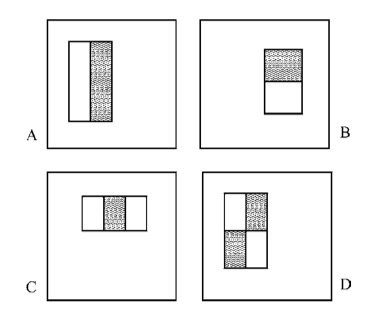
\includegraphics[scale=0.5]{features.jpg}
  \caption{Examples of features relative to the detection window}
  \label{fig:features}
\end{figure}

In order to make the implementation presented in this paper as close as possible
to the original algorithm described by Viola and Jones, features have been
calculated based only on the 2D RGB information of the point cloud. This makes
features calculation very fast and easy to reasonate about as the problem can be
modeled with simple two-dimensional array access. This means the point cloud
passed as input to the detector must be organized.

\subsection{Cascaded classifier}
Evaluation of a single feature is hardly sufficient to obtain a result that can
be distinguished by a random classifier operating over a uniform probability
distribution. A classifier operating with a single feature is termed for this
reason \emph{weak classifier}.

Given a detection window $x$, a feature $f$, a threshold $\theta$ and a polarity
$p$, a weak classifier can be described by the equation:

\[ 
  h(x,f,p,\theta) = 
\begin{cases}
  1,& \text{if } pf(x) < p\theta \\ 0,& \text{otherwise}
\end{cases}
\]

To obtain more robust results, weak classifiers can be combined together in a
linear combination. Such a combination is referred to as \emph{strong
classifier}. By means of a strong classifier it's possible to obtain
results that are satisfactory in terms of detection rate and false positive
rate, but at the expense of an increased need for computational power.

!! expand on strong classifier, put equation describing a strong classifier !!

To balance these two needs, a variant of the AdaBoost algorithm is introduced.

!! explain adaboost principles !!

\subsection{Integral image}
For efficient computation of features (both in detection and training), an
integral image representation of the original sample is computed.

In an integral image, each pixel is the sum of all the pixels above and to the
left.

\begin{figure}[h]
  \centering
  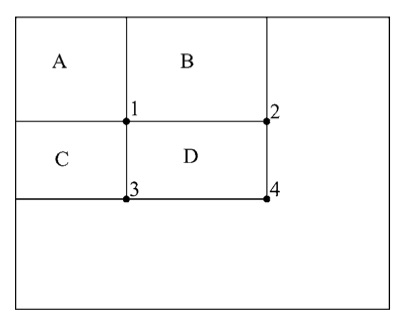
\includegraphics[scale=0.5]{area_sum_integral_image.jpg}
  \caption{The sum of the pixels within rectangle D can be computed with four
  array references: $4+1-2-3$}
  \label{fig:area_sum}
\end{figure}

Using this representation, the value of a rectangle area can be computed by 4
array references as illustrated in the picture above. Computing any of the
features described in the previous paragraph thus requires a constant number of
operations, independent from the size of the feature.

In practical terms, in order to perform all the required operations on an image
efficiently, we need to store both the integral image and the integral image of
the squares, that is the matrix in which each cell contains the square sum of
the cells above and to the left. This is needed in order to calculate the image
variance with $O(1)$ complexity.

Another interesting aspect of the implementation of the integral image is the
different way it is accessed by the training algorithm and the detection
algorithm. For the training algorithm all that's needed is to have an integral
image of the entire sample. A specific feature is calculated only once on the
overall sample. On the contrary, the detection algorithm needs to calculate
features multiple times across the same image. More importantly, image
normalization must happen on the overall sample in case of the training
algorithm, whereas in the detector each of the image portions scanned needs to
be normalized independently from the rest. \\
These two characteristics pose two problems: how to share the code that
calculates the integral image between the two use cases, and how to make image
normalization as efficient as possible.

The first problem has been solved by collecting the integral image and square
integral image calculation code in a common class named \texttt{IntegralImage}.
This class provides facilities to get various calculations for a specific
rectangle of the image held by a class' instance, such as the area sum, mean and
variance.  Taking it from there, then, in order to solve the second problem two
classes have been designed: \texttt{TrainingSample} and \texttt{SubWindow}. A
training sample maps the use case scenario found in training, which boils down
to simple area sum calculation using the whole integral image. A training sample
also stores information useful for the training itself, as for example a flag
saying if the sample contains a face or not (i.e. if it should be classified
positively or not). A sub-window, instead, maps the use case found in the
detector. The main feature is the possibility to calculate a feature on a
portion of the image that gets normalized independently from the rest of the
image.

Image normalization is required to make training and detection as independent as
possible from lighting conditions and general camera exposure. A form of
normalization useful in this case is variance normalization. This transforms the
input so that the end result has a $N(0,1)$ distribution.
Given a pixel value $x$ belonging to an image $X$, its variance-normalized
counterpart can be expressed as:

\[ x_{norm} = \dfrac{x - \overline{x}}{\sigma^{2}} \]

where $\overline{x}$ is the image's mean value, defined as:

\[ \overline{x} = \dfrac{1}{N} \sum X \]

whereas $\sigma^{2}$ is the square variance, defined as:

\[ \sigma^{2} = \overline{x}^{2} - \dfrac{1}{2} \sum X^{2} \]

We can then calculate the linear combination of a set of variance-normalized
pixels by relying on the following equation:

\[ \sum X_{norm} = \dfrac{\sum X}{\sigma^{2}} \]

We need then to solve the problem of how to efficiently calculate the value of a
feature normalized over a portion of the overall image. We do this by allowing a
\texttt{SubWindow} to be repositioned inside the original image. When
repositioning the sub-window, we recalculate the variance over the new image
portion. This is a step that requires $O(1)$ since the integral square image is
stored alongside with the integral image. At this point we can simply apply the
last equation whenever we calculate an area sum.

To make things easier, an instance of \texttt{SubWindow} stores the coordinates
of the image portion being analyzed (in the form of its top-left and
bottom-right corner). When repositioning the sub-window, we also recalculate and
store the variance of the image portion. By repositioning the sub-window instead
of the feature itself, we can achieve a consistent and position-independent
representation of a feature (i.e. the sub-window takes care of translating and
scaling the feature's coordinates).

\subsection{Sizing the features}
The original implementation of the Viola-Jones algorithm is designed to work on
2D images. This mean it doesn't accept any depth information. For this reason,
in the original papepr, the final detector needs to be run at different scales
in each area in order to take into account the fact that faces might be present
in different sizes. \\
In addition to that, a training algorithm has to focus on limited areas of a
specific scene. We'll call these areas \emph{samples}. The size of these samples
is also affected by the distance, and bears a direct linear relationship to the
size of the features. Determination of the size of a sample obeys the same rules
as the determination of a feature's size.

This extra computational step can be avoided if we consider depth information
present in a point cloud. In particular we can start from a reference sample
size, and then scale it based on the position on the Z-axis of the area of the
scene currently analyzed. \\
The reference sample should be big enough to guarantee it fits heads of any
size, but not any bigger. In other words, the reference sample should be as
small as possible without running into the risk of "cutting off" heads that
appear bigger because of camera distortion.

If the reference sample size is expressed for a sample lying on average 1m away
from the camera, then the size of any given sample can then be calculated just
by dividing the reference size by the sample distance.

In practical terms, this poses two problems: the fact that the calculation
happens on pixels and not of real values, and that the depth is not constant
over a specific area. \\
The first problem is simply solved by rounding up the division to the next
integer. Moreover, since once the sample size has been calculated we need to
calculate the precise pixel coordinates of the rectangle to consider, we take
the extra step of rounding up the upper coordinates (i.e. bottom-right corner),
while at the same time we round down the lower coordinates (i.e. top-left
corner). This ensures that even at a big distance we minimize the effect of
rounding by oversizing the sample square.

The problem of the distance not being constant over an area is solved by always
considering the point being analyzed as the center of a rectangle. While this
seems overly simplistic, we also leverage the sequential scanning of the image.
Given that the reference sample is sized so that small variations in the final
sample size don't affect the detector's performance, if at a certain point we
encounter an outlier (either a NaN or a point with a lot of noise in the
distance information), we can just assume that at least one of its neighbors
contains correct information. In other words, in case we encounter outliers, we
can safely assume that the algorithm already classified or will classify the
area correctly when analyzing neighbor points. \\
The only downside of this approach is that in case of area that are overall
noisy (such as peripheral areas in the camera's field of view) the algorithm
might end up skipping classification on large portions of the image. But in that
case, classification is generally difficult anyway given the low SNR.

Another small inefficiency present in the scanning loop due to this
approximation of an area's average distance is the computation that happens at
the boundaries of the scene. Since a specific point is considered the center of
a square when determining the sample size and position, there must be enough
points in all directions so that a full square can be extracted and analyzed. If
the scanning algorithm is working near the image's boundaries, this condition
might not be respected. In this case, the algorithm also skips detection, based
on the assumption that at some point the same algorithm will analyze a close
neighbor whose distance will allow to include all the points discarded up to
that point because the sample would overflow.

The calculation of the size of a feature is performed on a similar basis but
with a caveat: each feature needs to record additional information relative to
the size of the sample that was used when training it. This is necessary because
by introducing information about image depth in the training algorithm, a
specific feature's size loses all meanings when the feature needs to be
rescaled, if the same information is not related to the size of the sample it
was trained with.

In addition to the point above, depth information is also used to minimize the
amount of features generated and evaluated when training the classifier. In the
2D version of the algorithm, all features of all size from 1x1 to the size of
the image must be generated. In the case of a 3D point cloud, we can reduce the
amount of features to those that fit the smallest sample present in the scene.
Features for bigger samples can be upscaled from the smaller ones. This approach
offer two contrasting aspects:

\begin{itemize}
  \item on one side, resolution is lost when upscaling the features (the bigger the
  size differences among samples, the bigger the loss)
  \item on the other side, starting from a set of features for a bigger sample, opens
  the door to the risk of downscaling a feature to the point it goes to a
  sub-pixel level, resulting in a complete loss of informaton during the training
  process.
\end{itemize}

Trials on the designed algorithm showed that the problem introduced by
downsampling features to sub-pixel sizes was jeopardizing the algorithm's
effectiveness, so the first option was selected.

\section{Body segmentation}

\section{Implementation details}
tool to extract faces
training application
detector


\section{Results}

\section{Further developments}
* better algorithm training to remove the need of additional processing
* different measurements can be used to calculate features (e.g. face depth map)
* parallelization of feature values calculation for even faster implementation
* combination of multiple, parallel detectors to improve detection performance
  and allow a wider range of poses to be identified (e.g. profile detector)
* use of color information to improve detection performance (human skin lies in
  a restricted range of color variations)
* adaptation of the algorithm to take advantage of moving targets (i.e.
  implementation of a companion tracking algorithm)

\end{document}
